%% State Space Modelling of Dynamic Systems
%% Lecture 19: Controllability and Observability
\def\FileDate{10/02/01}
\def\FileVersion{1.0}
% ----------------------------------------------------------------
% Notes pages *********************************************************
% ----------------------------------------------------------------

We now turn our attention to the design of control systems using stats space techniques. The idea is that we measure the state of the system in some way and adjust the inputs to modify the state behaviour. However this implies that we can both \emph{observe} the states and \emph{control} them. This section introduces the basic concept of observability and controllability.

The development of state space system models led to clarification of the issues of controllability and observability.

In classical control system theory, which is based on transfer functions, there is really no equivalent concept.

\section{System Partitioning} % (fold)
\label{sec:system_partitioning}

Imagine a system with a set of inputs feeding a set of state equations which in turn generate a set of outputs.

The state equations may be partitioned into four subsets forming sub-systems, $\mathbf{S1}$, $\mathbf{S2}$, $\mathbf{S3}$ and $\mathbf{S4}$. 

(Some of the sets may be empty depending on the extent of the system controllability and/or observability)


\begin{center}
	\resizebox{200pt}{!}{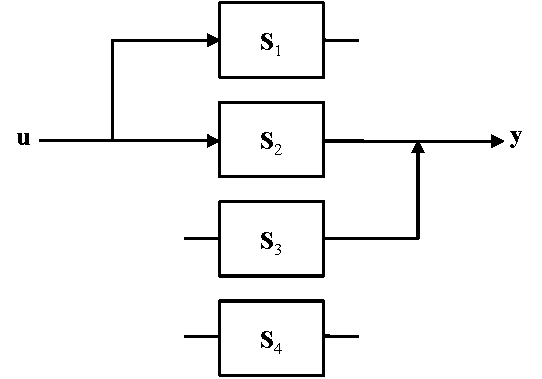
\includegraphics{pictures/partitioning.pdf}}
\end{center}
\endinput

%%% Local Variables: 
%%% mode: latex
%%% TeX-master: "notes"
%%% End:
\ifslidesonly
\begin{slide}
   \heading{System Partitioning}
   
\begin{center}
	\resizebox{200pt}{!}{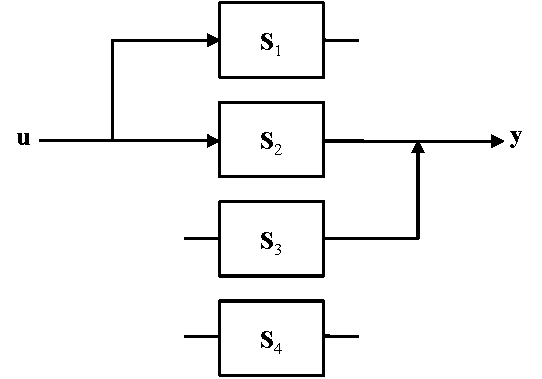
\includegraphics{pictures/partitioning.pdf}}
\end{center}
\endinput

%%% Local Variables: 
%%% mode: latex
%%% TeX-master: "notes"
%%% End:
\end{slide}
\fi

If a sub-system is connected to the inputs $\mathbf{u}$ then it is said to be \emph{controllable}. That is, we can control the states of that sub-system from the inputs. Conversely, if there is no connection, then we cannot influence those states from the inputs and the sub-system is \emph{uncontrollable}.

Similarly, if a sub-system is connected to the outputs $\mathbf{y}$ then it is said to be \emph{observable}. That is, we can observe or measure the states of that sub-system from a knowledge of the output values. Conversely, if there is no connection, then there is no information about those states contained in the outputs and the sub-system is \emph{unobservable}.
\ifslidesonly
\begin{slide}
   \heading{Controllability}
\begin{itemize}
	\item If a sub-system is connected to the inputs $\mathbf{u}$ then it is said to be \emph{controllable}. 
	\item If there is no connection the sub-system is \emph{uncontrollable}.
	\item If a sub-system is connected to the outputs $\mathbf{y}$ then it is said to be \emph{observable}. 
	\item If there is no connection the sub-system is \emph{unobservable}.
\end{itemize}
\end{slide}
\fi
 
% section system_partitioning (end)

\section*{Controllability and observability of the sub-systems} % (fold)
\label{sec:section_name}

Given the transformation $\mathbf{T}^{-1}\mathbf{AT}=\mathbf{\Lambda}$:
\begin{eqnarray*}
	\mathbf{A}t & = & (\mathbf{T\Lambda T}^{-1}) t \\
	\mathbf{A}^nt^n & = & (\mathbf{T\Lambda T}^{-1})(\mathbf{T\Lambda T}^{-1})\ldots(\mathbf{T\Lambda T}^{-1})t^n \\
	                & = & \mathbf{T\Lambda T}^{-1}\mathbf{T\Lambda T}^{-1}\ldots\mathbf{T\Lambda T}^{-1}t^n \\
	\mathbf{A}^nt^n & = & \mathbf{T\Lambda}\mathbf{I}\mathbf{\Lambda I}\ldots\mathbf{I\Lambda T}^{-1}t^n \\
	\               & = & \mathbf{T\Lambda}^n\mathbf{T}^{-1}t^n \\
\end{eqnarray*}
\endinput

%%% Local Variables: 
%%% mode: latex
%%% TeX-master: "notes"
%%% End:
\ifslidesonly
\begin{slide}
   \heading{Controllability and observability of the sub-systems}
   Given the transformation $\mathbf{T}^{-1}\mathbf{AT}=\mathbf{\Lambda}$:
\begin{eqnarray*}
	\mathbf{A}t & = & (\mathbf{T\Lambda T}^{-1}) t \\
	\mathbf{A}^nt^n & = & (\mathbf{T\Lambda T}^{-1})(\mathbf{T\Lambda T}^{-1})\ldots(\mathbf{T\Lambda T}^{-1})t^n \\
	                & = & \mathbf{T\Lambda T}^{-1}\mathbf{T\Lambda T}^{-1}\ldots\mathbf{T\Lambda T}^{-1}t^n \\
	\mathbf{A}^nt^n & = & \mathbf{T\Lambda}\mathbf{I}\mathbf{\Lambda I}\ldots\mathbf{I\Lambda T}^{-1}t^n \\
	\               & = & \mathbf{T\Lambda}^n\mathbf{T}^{-1}t^n \\
\end{eqnarray*}
\endinput

%%% Local Variables: 
%%% mode: latex
%%% TeX-master: "notes"
%%% End:
\end{slide}
\fi


If sub-sets $\mathbf{S}_3$ and $\mathbf{S}_4$ are empty then the entire system is completely controllable.

If sub-sets $\mathbf{S}_1$ and $\mathbf{S}_4$ are empty then the entire system is completely observable.


% section Controllability_and_observability_of_the_sub-systems (end)

\section*{Mathematical Test for Controllability} % (fold)
\label{sec:mathematical_test_for_controllability}


If we transform the state equations to normal canonical form, then the term involving the inputs constitutes the link in the previous figure between $\mathbf{u}$ and the sub-systems.

From previous work we had:
\[
\dot{\mathbf{x}} = \mathbf{Ax} + \mathbf{Bu}
\]
with state transformation matrix $\mathbf{T}$ giving:
\begin{eqnarray*}
	\mathbf{x} & = & \mathbf{Tw} \\
	\dot{\mathbf{w}}& = &\mathbf{T}^{-1}\mathbf{ATw}+\mathbf{T}^{-1}\mathbf{Bu} \\
	& = & \mathbf{\Lambda w}= \mathbf{T}^{-1}\mathbf{Bw}
\end{eqnarray*}
where $\mathbf{\Lambda}$ is a diagonal matrix.
 
For controllability of all the system states, every state equation must be linked to at least one of the inputs. The $i^\mathrm{th}$ state equation is:
\[
\dot{w}_i = \lambda_iw_i + \left[i^{\mathrm{th}}\mathrm{\ row\ of\ }\mathbf{T}^{-1}\mathbf{B}\right]\mathbf{u}
\]
 
Therefore for every state equation to be linked to at least one input, there must be no row of $\mathbf{T}^{-1}\mathbf{B}$  containing all zero entries.
\ifslidesonly
\begin{slide}
   \heading{Mathematical Test for Controllability (1)}
   If we transform the state equations to normal canonical form, then the term involving the inputs constitutes the link in the previous figure between $\mathbf{u}$ and the sub-systems.

From previous work we had:
\[
\dot{\mathbf{x}} = \mathbf{Ax} + \mathbf{Bu}
\]
with state transformation matrix $\mathbf{T}$ giving:
\begin{eqnarray*}
	\mathbf{x} & = & \mathbf{Tw} \\
	\dot{\mathbf{w}}& = &\mathbf{T}^{-1}\mathbf{ATw}+\mathbf{T}^{-1}\mathbf{Bu} \\
	& = & \mathbf{\Lambda w}= \mathbf{T}^{-1}\mathbf{Bw}
\end{eqnarray*}
where $\mathbf{\Lambda}$ is a diagonal matrix.
\end{slide}

\begin{slide}
   \heading{Mathematical Test for Controllability (2)}
\begin{itemize}
	\item For controllability of all the system states, every state equation must be linked to at least one of the inputs.
	\item  The $i^\mathrm{th}$ state equation is:
	\[
	\dot{w}_i = \lambda_iw_i + \left[i^{\mathrm{th}}\mathrm{\ row\ of\ }\mathbf{T}^{-1}\mathbf{B}\right]\mathbf{u}
	\]
	\item Therefore for every state equation to be linked to at least one input, there must be no row of $\mathbf{T}^{-1}\mathbf{B}$  containing all zero entries.
\end{itemize}

\end{slide}
\fi


% section mathematical_test_for_controllability (end)

\section{Mathematical Test for Observability} % (fold)
\label{sec:mathematical_test_for_observability}

If we transform the output equations to normal canonical form, then the term involving the states constitutes the link in the previous figure between the sub-system states and outputs $\mathbf{y}$.

From previous work we had:
\[
\mathbf{y} = \mathbf{Cx} + \mathbf{Du}
\]
 
Transforming to normal canonical form with matrix $\mathbf{T}$ gives:
\begin{eqnarray*}
	\mathbf{x} & = & \mathbf{Tw} \\
	\mathbf{y}& = &\mathbf{CTw}+\mathbf{Du} \\
\end{eqnarray*}

For observability of all the system states, every state $w_i$ must be linked to at least one of the outputs.  Therefore, there must be no column of $\mathbf{CT}$  containing all zero entries.
\ifslidesonly
\begin{slide}
   \heading{Mathematical Test for Observability (1)}
If we transform the output equations to normal canonical form, then the term involving the states constitutes the link in the previous figure between the sub-system states and outputs $\mathbf{y}$.

From previous work we had:
\[
\mathbf{y} = \mathbf{Cx} + \mathbf{Du}
\]

Transforming to normal canonical form with matrix $\mathbf{T}$ gives:
\begin{eqnarray*}
	\mathbf{x} & = & \mathbf{Tw} \\
	\mathbf{y}& = &\mathbf{CTw}+\mathbf{Du} \\
\end{eqnarray*}
\end{slide}
\begin{slide}
   \heading{Mathematical Test for Observability (2)}
\begin{itemize}
	\item For observability of all the system states, every state $w_i$ must be linked to at least one of the outputs.
	\item Therefore, there must be no column of $\mathbf{CT}$  containing all zero entries.   
\end{itemize}
\end{slide}
\fi

The previous arguments have indicated necessary conditions for controllability and observability but even if they are true they do not give a guarantee. Sufficient conditions require more subtle tests as quoted in the next section.


% section mathematical_test_for_observability (end)

\section*{Alternative Tests for Controllability and Observability} % (fold)
\label{sec:alternative_tests_for_controllability_and_observability}

To apply the tests of the previous sections involves deriving the transformation matrix $\mathbf{T}$, the columns of which consist of the eigenvectors of the original state matrix $\mathbf{A}$. It is not necessary to form $\mathbf{T}$ explicitly and alternative tests exist based on the untransformed matrices $\mathbf{A}$, $\mathbf{B}$ and $\mathbf{C}$ only.

For an $n^{\mathrm{th}}$ order system, the system is completely \emph{state controllable} if the \textbf{controllability matrix}:
\[
\left[\mathbf{B}\vdots\mathbf{AB}\vdots\cdots\vdots\mathbf{A}^{n-1}\mathbf{B}\right]
\]
is of rank $n$. (i.e. it contains $n$ linearly independent rows or, in other words, its determinant is non-zero.)

Similarly, a system is completely \emph{state observable} if the \textbf{observability matrix}
\[
\left[\mathbf{C}^T\vdots\mathbf{A}^T\mathbf{C}^T\vdots\cdots\vdots\left(\mathbf{A}^T\right)^{n-1}\mathbf{C}^T\right]
\]
is of rank $n$ (i.e. its determinant is non-zero.)

These two conditions can result in numerically ill-conditioned calculations for large $n$.

\ifslidesonly
\begin{slide}
   \heading{Alternative tests: Controllability}
   For an $n^{\mathrm{th}}$ order system, the system is completely \emph{state controllable} if the \textbf{controllability matrix}:
\[
\left[\mathbf{B}\vdots\mathbf{AB}\vdots\cdots\vdots\mathbf{A}^{n-1}\mathbf{B}\right]
\]
is of rank $n$.
\end{slide}

\begin{slide}
\heading{Alternative tests: Observability}
For an $n^{\mathrm{th}}$ order system, a system is completely \emph{state observable} if the \textbf{observability matrix}
\[
\left[\mathbf{C}^T\vdots\mathbf{A}^T\mathbf{C}^T\vdots\cdots\vdots\left(\mathbf{A}^T\right)^{n-1}\mathbf{C}^T\right]
\]
is of rank $n$.
\end{slide}
\fi

\subsection*{Example} % (fold)
\label{sub:example}

\textbf{Problem}: test the following system for controllability and observability:
\begin{eqnarray*}
	 {\bf{\dot x}}  & = &   \left[ {\begin{array}{*{20}c}
	   { - 6} & { - 5}  \\
	   1 & 0  \\
	\end{array}} \right]{\bf{x}} + \left[ {\begin{array}{*{20}c}
	   1  \\
	   0  \\
	\end{array}} \right]u \\
		 y & = &  \left[ {\begin{array}{*{20}c}
	   3 & 1  \\
	\end{array}} \right]{\bf{x}} \\ 
\end{eqnarray*}


\textbf{SOLUTION}:
% MathType!MTEF!2!1!+-
% faaagaart1ev2aaaKnaaaaWenf2ys9wBH5garuavP1wzZbqedmvETj
% 2BSbqefm0B1jxALjharqqtubsr4rNCHbGeaGqiVu0Je9sqqrpepC0x
% bbL8FesqqrFfpeea0xe9Lq-Jc9vqaqpepm0xbba9pwe9Q8fs0-yqaq
% pepae9pg0FirpepeKkFr0xfr-xfr-xb9Gqpi0dc9adbaqaaeGaciGa
% aiaabeqaamaabaabaaGcbaGaaCOqaiabg2da9maadmaabaqbamqabi
% qaaaqaaiaaigdaaeaacaaIWaaaaaGaay5waiaaw2faaiaacUdacaaM
% f8UaaCyqaiaahkeacqGH9aqpdaWadaqaauaadeqaciaaaeaacqGHsi
% slcaaI2aaabaGaeyOeI0IaaGynaaqaaiaaigdaaeaacaaIWaaaaaGa
% ay5waiaaw2faamaadmaabaqbamqabiqaaaqaaiaaigdaaeaacaaIWa
% aaaaGaay5waiaaw2faaiabg2da9maadmaabaqbamqabiqaaaqaaiab
% gkHiTiaaiAdaaeaacaaIXaaaaaGaay5waiaaw2faaaaa!47F8!
\[
{\bf{B}} = \left[ {\begin{array}{*{20}c}
   1  \\
   0  \\
\end{array}} \right];\quad {\bf{AB}} = \left[ {\begin{array}{*{20}c}
   { - 6} & { - 5}  \\
   1 & 0  \\
\end{array}} \right]\left[ {\begin{array}{*{20}c}
   1  \\
   0  \\
\end{array}} \right] = \left[ {\begin{array}{*{20}c}
   { - 6}  \\
   1  \\
\end{array}} \right]
\]

Therefore the determinant of the controllability matrix is:
% MathType!MTEF!2!1!+-
% faaagaart1ev2aaaKnaaaaWenf2ys9wBH5garuavP1wzZbqedmvETj
% 2BSbqefm0B1jxALjharqqtubsr4rNCHbGeaGqiVu0Je9sqqrpepC0x
% bbL8FesqqrFfpeea0xe9Lq-Jc9vqaqpepm0xbba9pwe9Q8fs0-yqaq
% pepae9pg0FirpepeKkFr0xfr-xfr-xb9Gqpi0dc9adbaqaaeGaciGa
% aiaabeqaamaabaabaaGcbaGaciizaiaacwgacaGG0bWaamWaaeaafa
% WabeGacaaabaGaaGymaaqaaiabgkHiTiaaiAdaaeaacaaIWaaabaGa
% aGymaaaaaiaawUfacaGLDbaacqGH9aqpcaaIXaGaeyOeI0Iaaiikai
% abgkHiTiaaiAdacqGHxdaTcaaIWaGaaiykaiabg2da9iaaigdacqGH
% GjsUcaaIWaaaaa!4385!
\[
\det \left[ {\begin{array}{*{20}c}
   1 & { - 6}  \\
   0 & 1  \\
\end{array}} \right] = 1 - ( - 6 \times 0) = 1 \ne 0
\]
Therefore the system is controllable.
 
\[
{\bf{C}^T} = \left[ {\begin{array}{*{20}c}
   3  \\
   1  \\
\end{array}} \right];\quad {\bf A}^T{\bf C}^T = \left[ {\begin{array}{*{20}c}
   { - 6} & { - 5}  \\
   1 & 0  \\
\end{array}} \right]\left[ {\begin{array}{*{20}c}
   3  \\
   1  \\
\end{array}} \right] = \left[ {\begin{array}{*{20}c}
   { -17 }  \\
   { -15 }  \\
\end{array}} \right]
\]

Therefore the determinant of the observability matrix is:
\[
\det \left[ {\begin{array}{*{20}c}
   3 & { -17 }  \\
   1 & { -15 }  \\
\end{array}} \right] = 3\times(-15) - (-17) \times 1) = -28 \ne 0
\]
Therefore the system is observable.

% subsection example (end)Test the following system for controllability and observability:

\subsection{Exercise} % (fold)
\label{sub:exercise}

Confirm these results by using system transformation to normal form.

% subsection exercise (end)


 


% section alternative_tests_for_controllability_and_observability (end)


\section*{Matlab functions} % (fold)
\label{sec:matlab_functions}

\begin{slide}
   \heading{Matlab function for testing controllability}
\begin{verbatim}
A = [-6 -5; 1 0];
B = [1; 0]
CM = ctrb(A, B)
rank(CM) % should be 2.
\end{verbatim}
\textbf{Important note}: \texttt{ctrb} is not recommended for serious control design use as it is numerically unstable.
\end{slide}

\begin{slide}
   \heading{Matlab function for testing observability}
\begin{verbatim}
A = [-6 -5; 1 0];
C = [3 1]
OM = obsv(A, C)
rank(OM) % should be 2.
\end{verbatim}
\textbf{Important note}: \texttt{obsv} is not recommended for serious control design use as it is numerically unstable.
\end{slide}

\begin{slide}
   \heading{Observability/controllability of systems}
\begin{verbatim}
A = [-6 -5; 1 0]; B = [1; 0]
C = [3 1];
sys = ss(A, B, C);
OM = obsv(sys)
CM = ctrb(sys)
\end{verbatim}
\end{slide}
% section matlab_functions (end)






%----------------------------------------------------------------
% The end of notes
% ----------------------------------------------------------------
\endinput

%%% Local Variables: 
%%% mode: latex
%%% TeX-master: t
%%% End: 
